\chapter{Beispiele}

Der User startet den Bot via dem Klick auf einen Link, den er auf einer Website findet oder der ihm zugesandt wird.

\subsection{Stage 00}
/start
\begin{figure} %[hbtp]
	\centering
	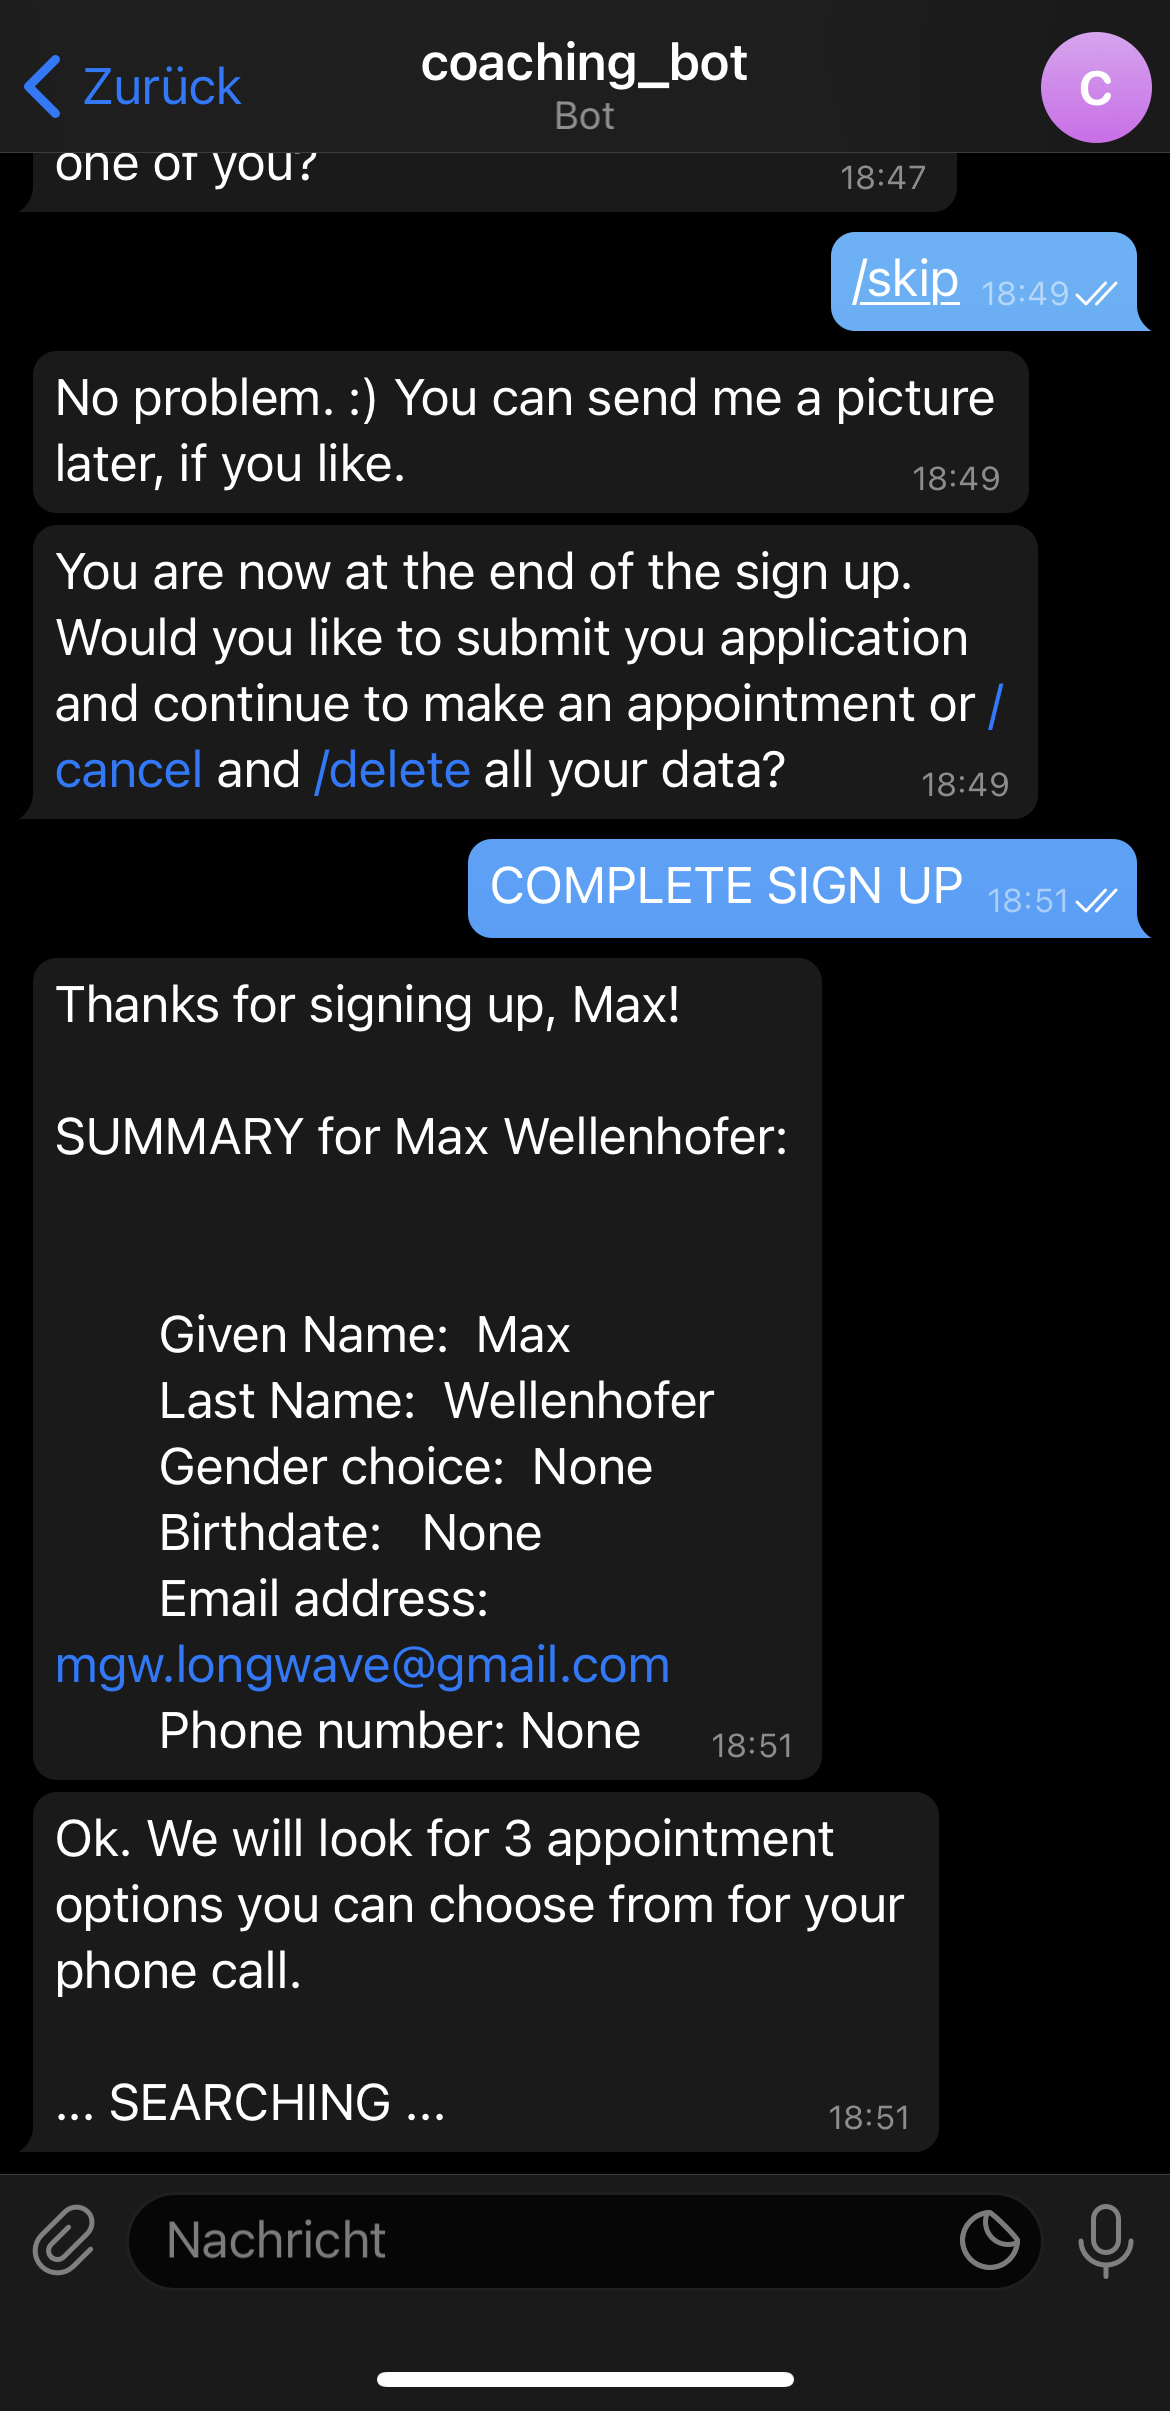
\includegraphics{images/coaching_bot_dummy_screenshot.jpeg}
	\caption{Bezeichnung der Abbildung}
	\label{a1}
\end{figure}


\subsection{Stage 01}
\begin{figure} %[hbtp]
	\centering
	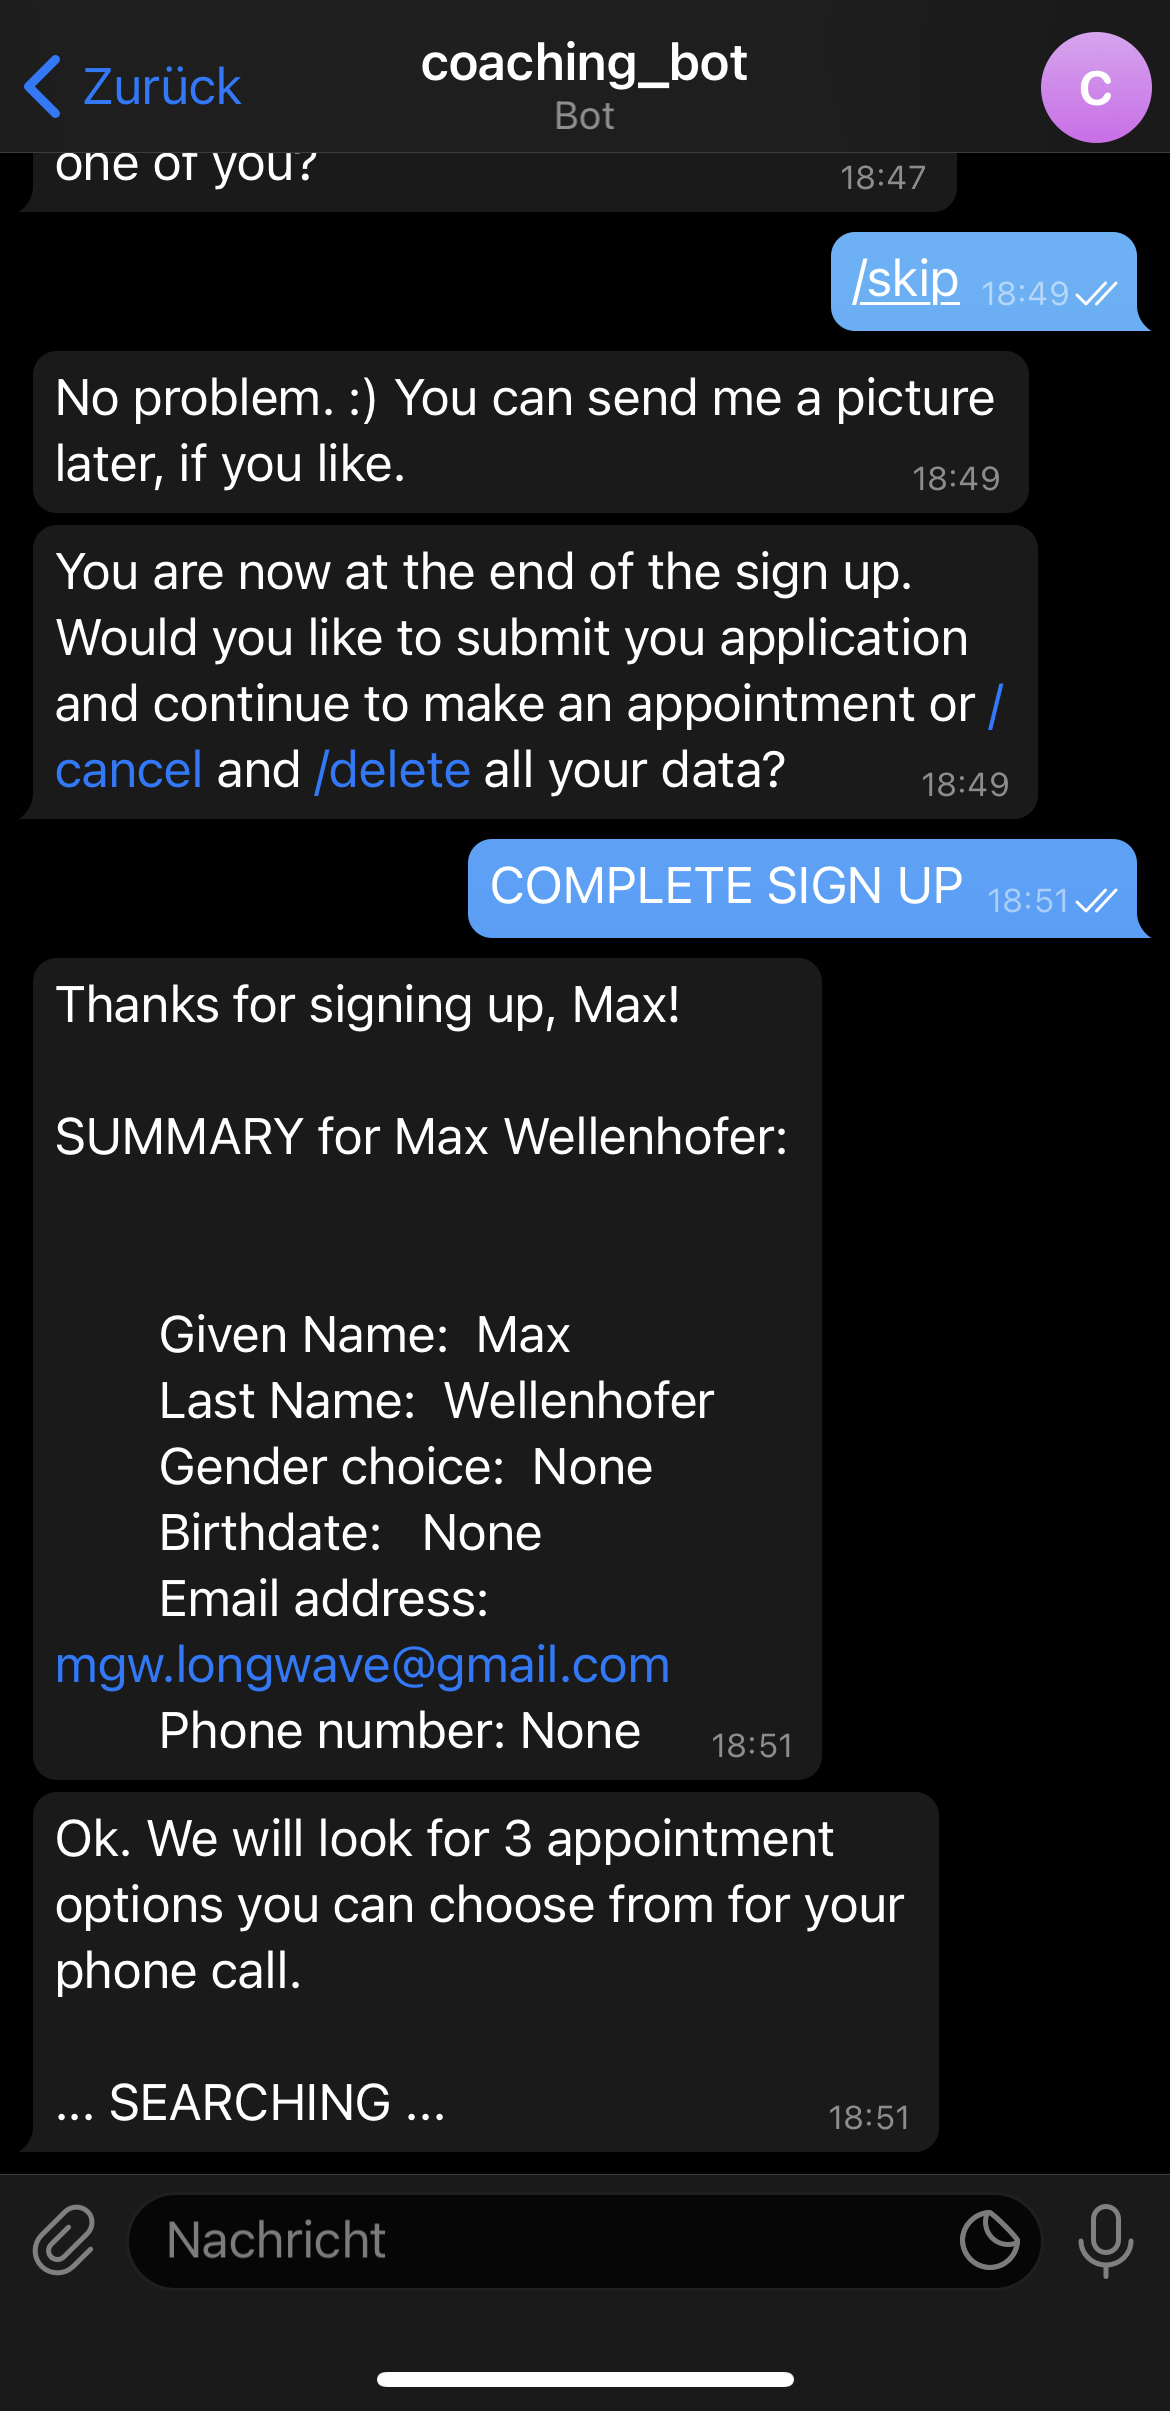
\includegraphics{images/coaching_bot_dummy_screenshot.jpeg}
	\caption{Bezeichnung der Abbildung}
	\label{a2}
\end{figure}


\subsection{Stage 02}
\begin{figure} %[hbtp]
	\centering
	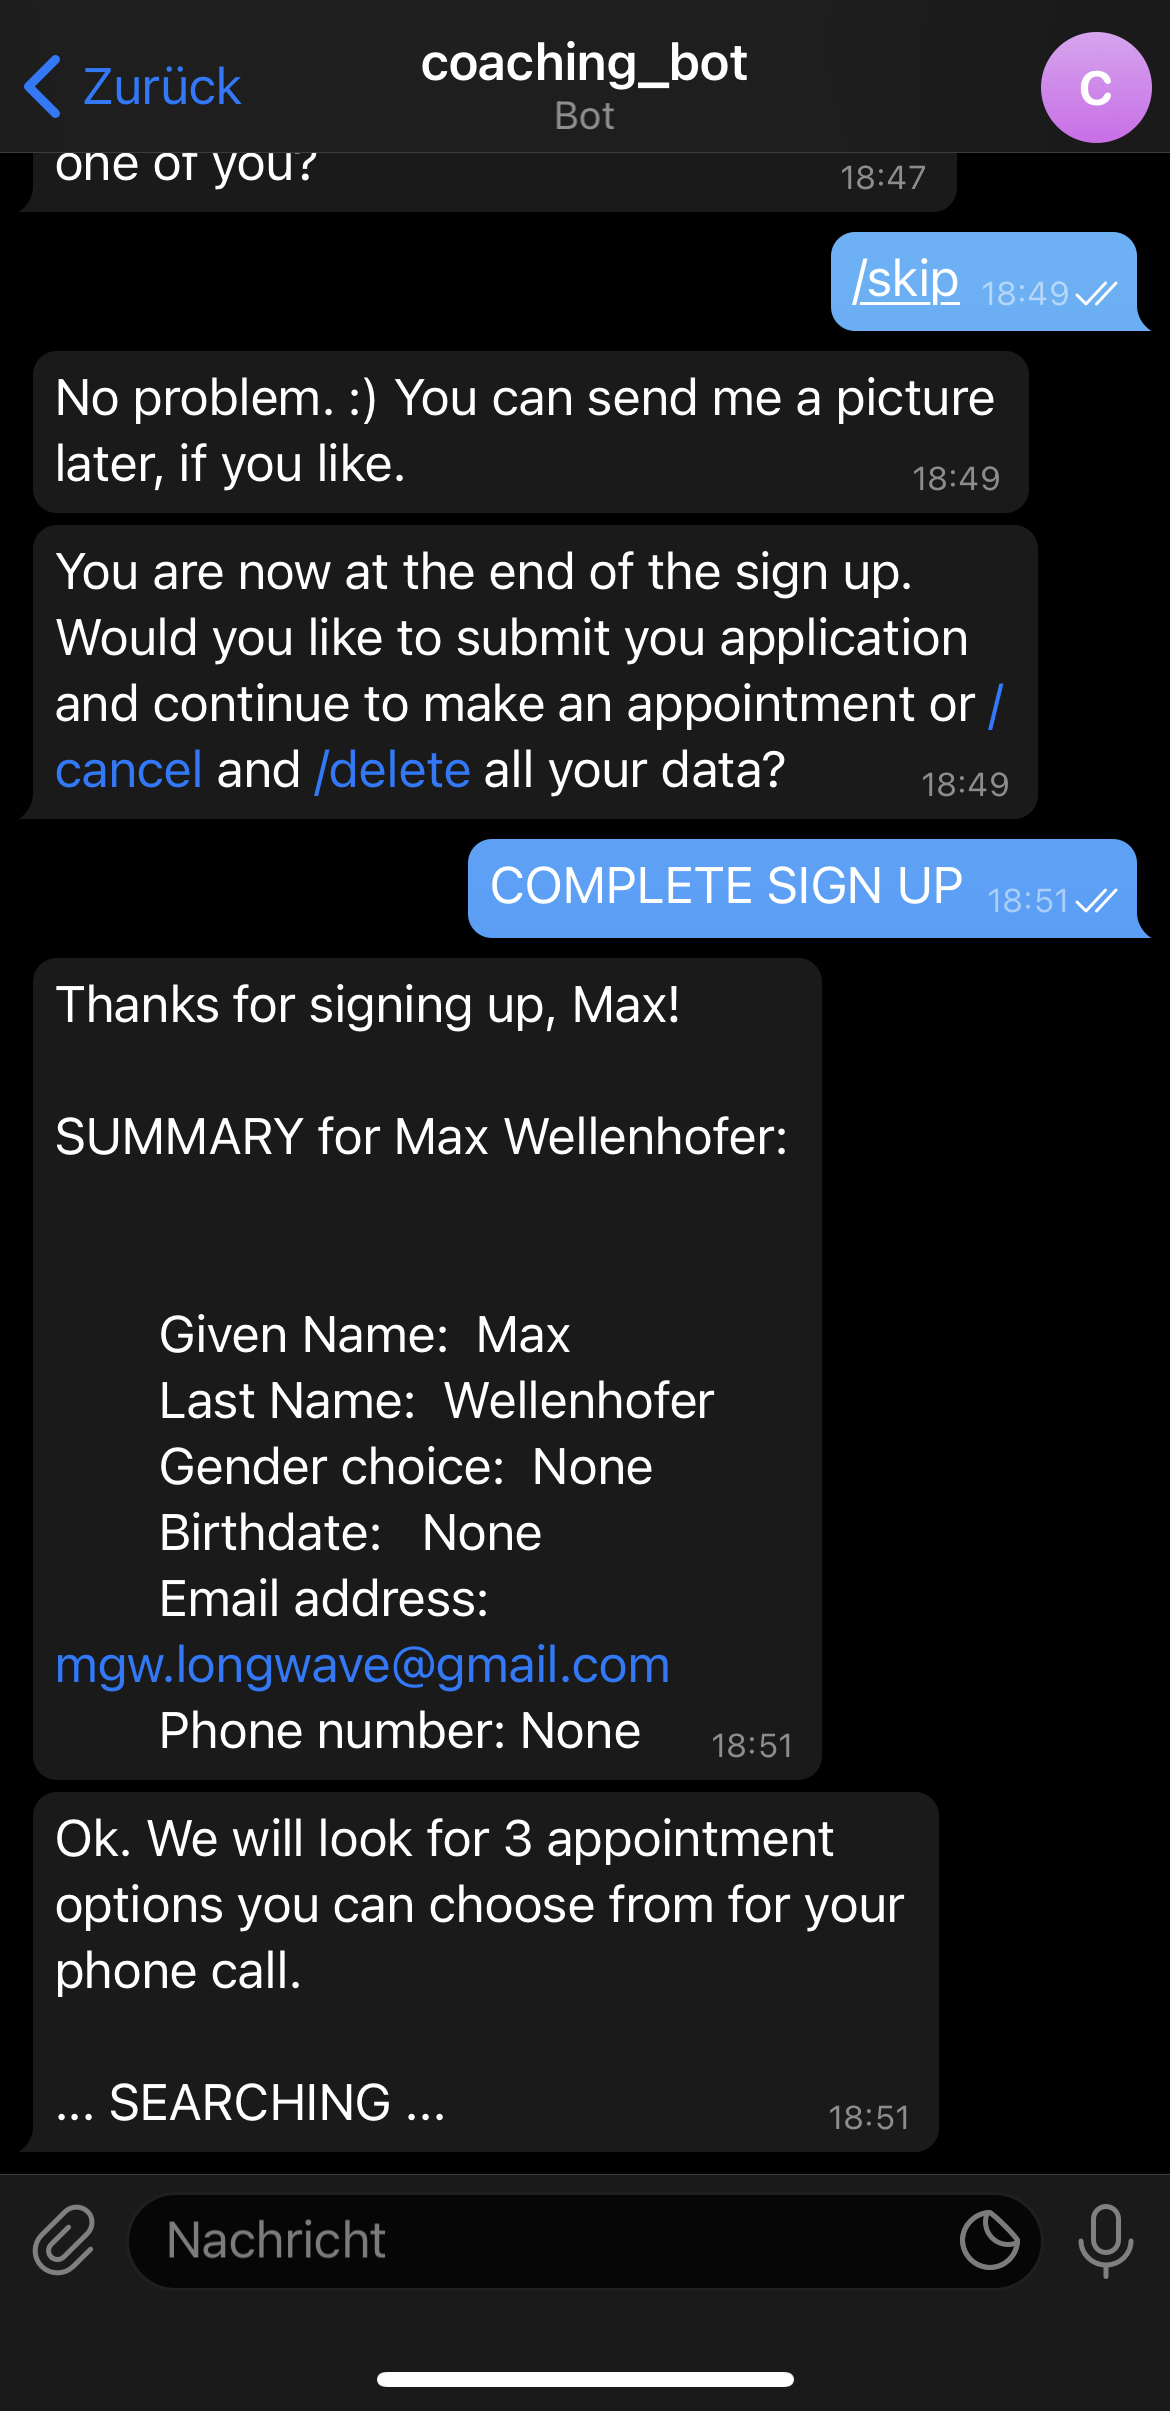
\includegraphics{images/coaching_bot_dummy_screenshot.jpeg}
	\caption{Bezeichnung der Abbildung}
	\label{a3}
\end{figure}


\subsection{Stage 03}
\begin{figure} %[hbtp]
	\centering
	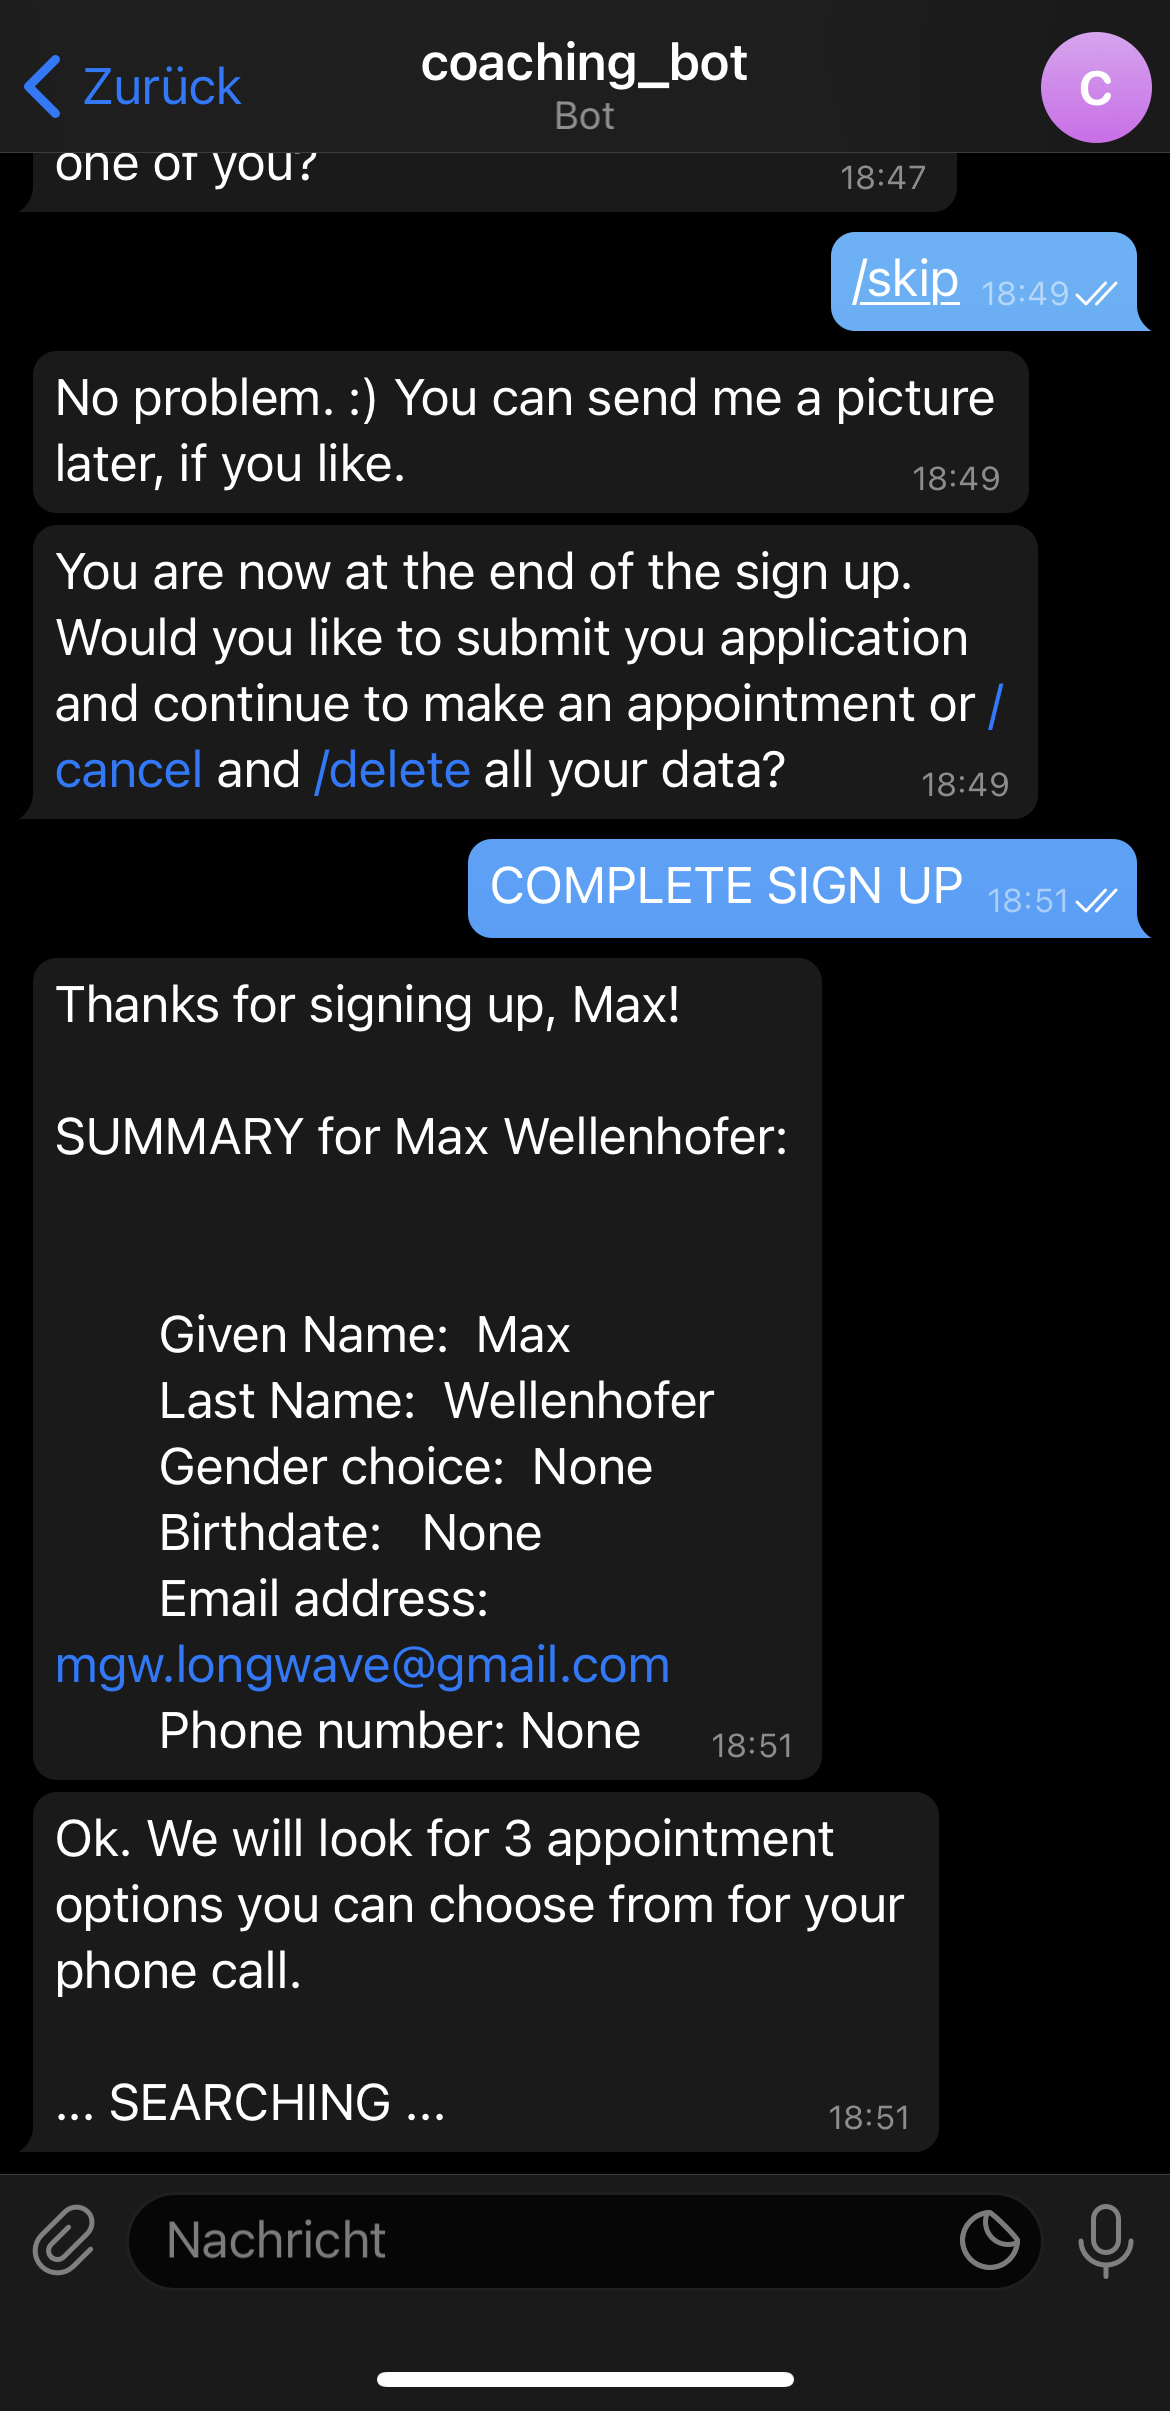
\includegraphics{images/coaching_bot_dummy_screenshot.jpeg}
	\caption{Bezeichnung der Abbildung}
	\label{a4}
\end{figure}


\subsection{Stage 04}
\begin{figure} %[hbtp]
	\centering
	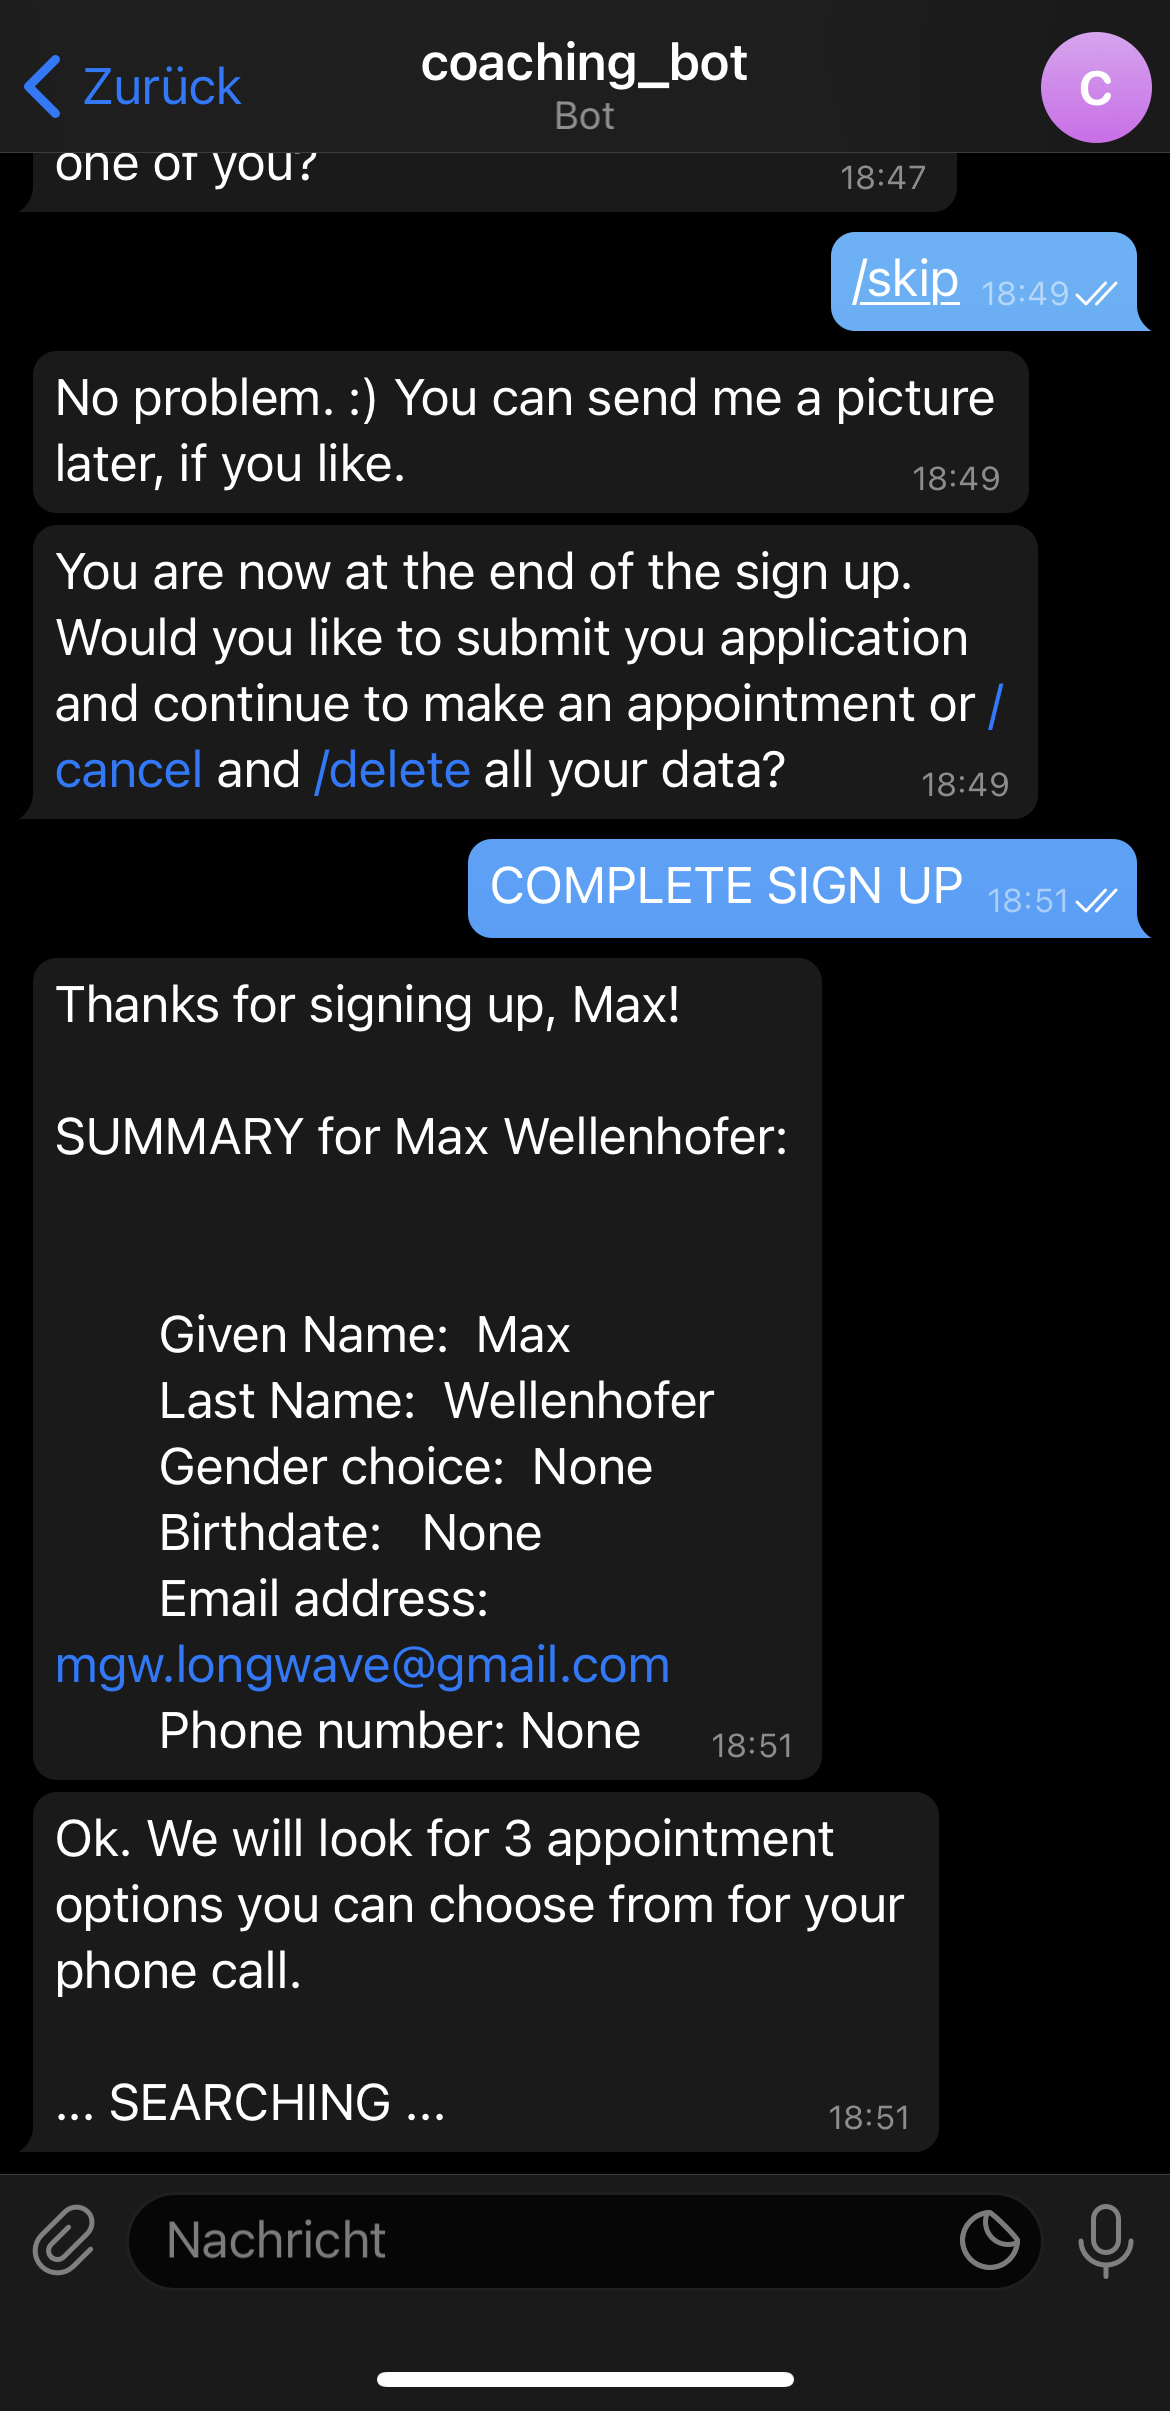
\includegraphics{images/coaching_bot_dummy_screenshot.jpeg}
	\caption{Bezeichnung der Abbildung}
	\label{a5}
\end{figure}


\subsection{Stage 05}
\begin{figure} %[hbtp]
	\centering
	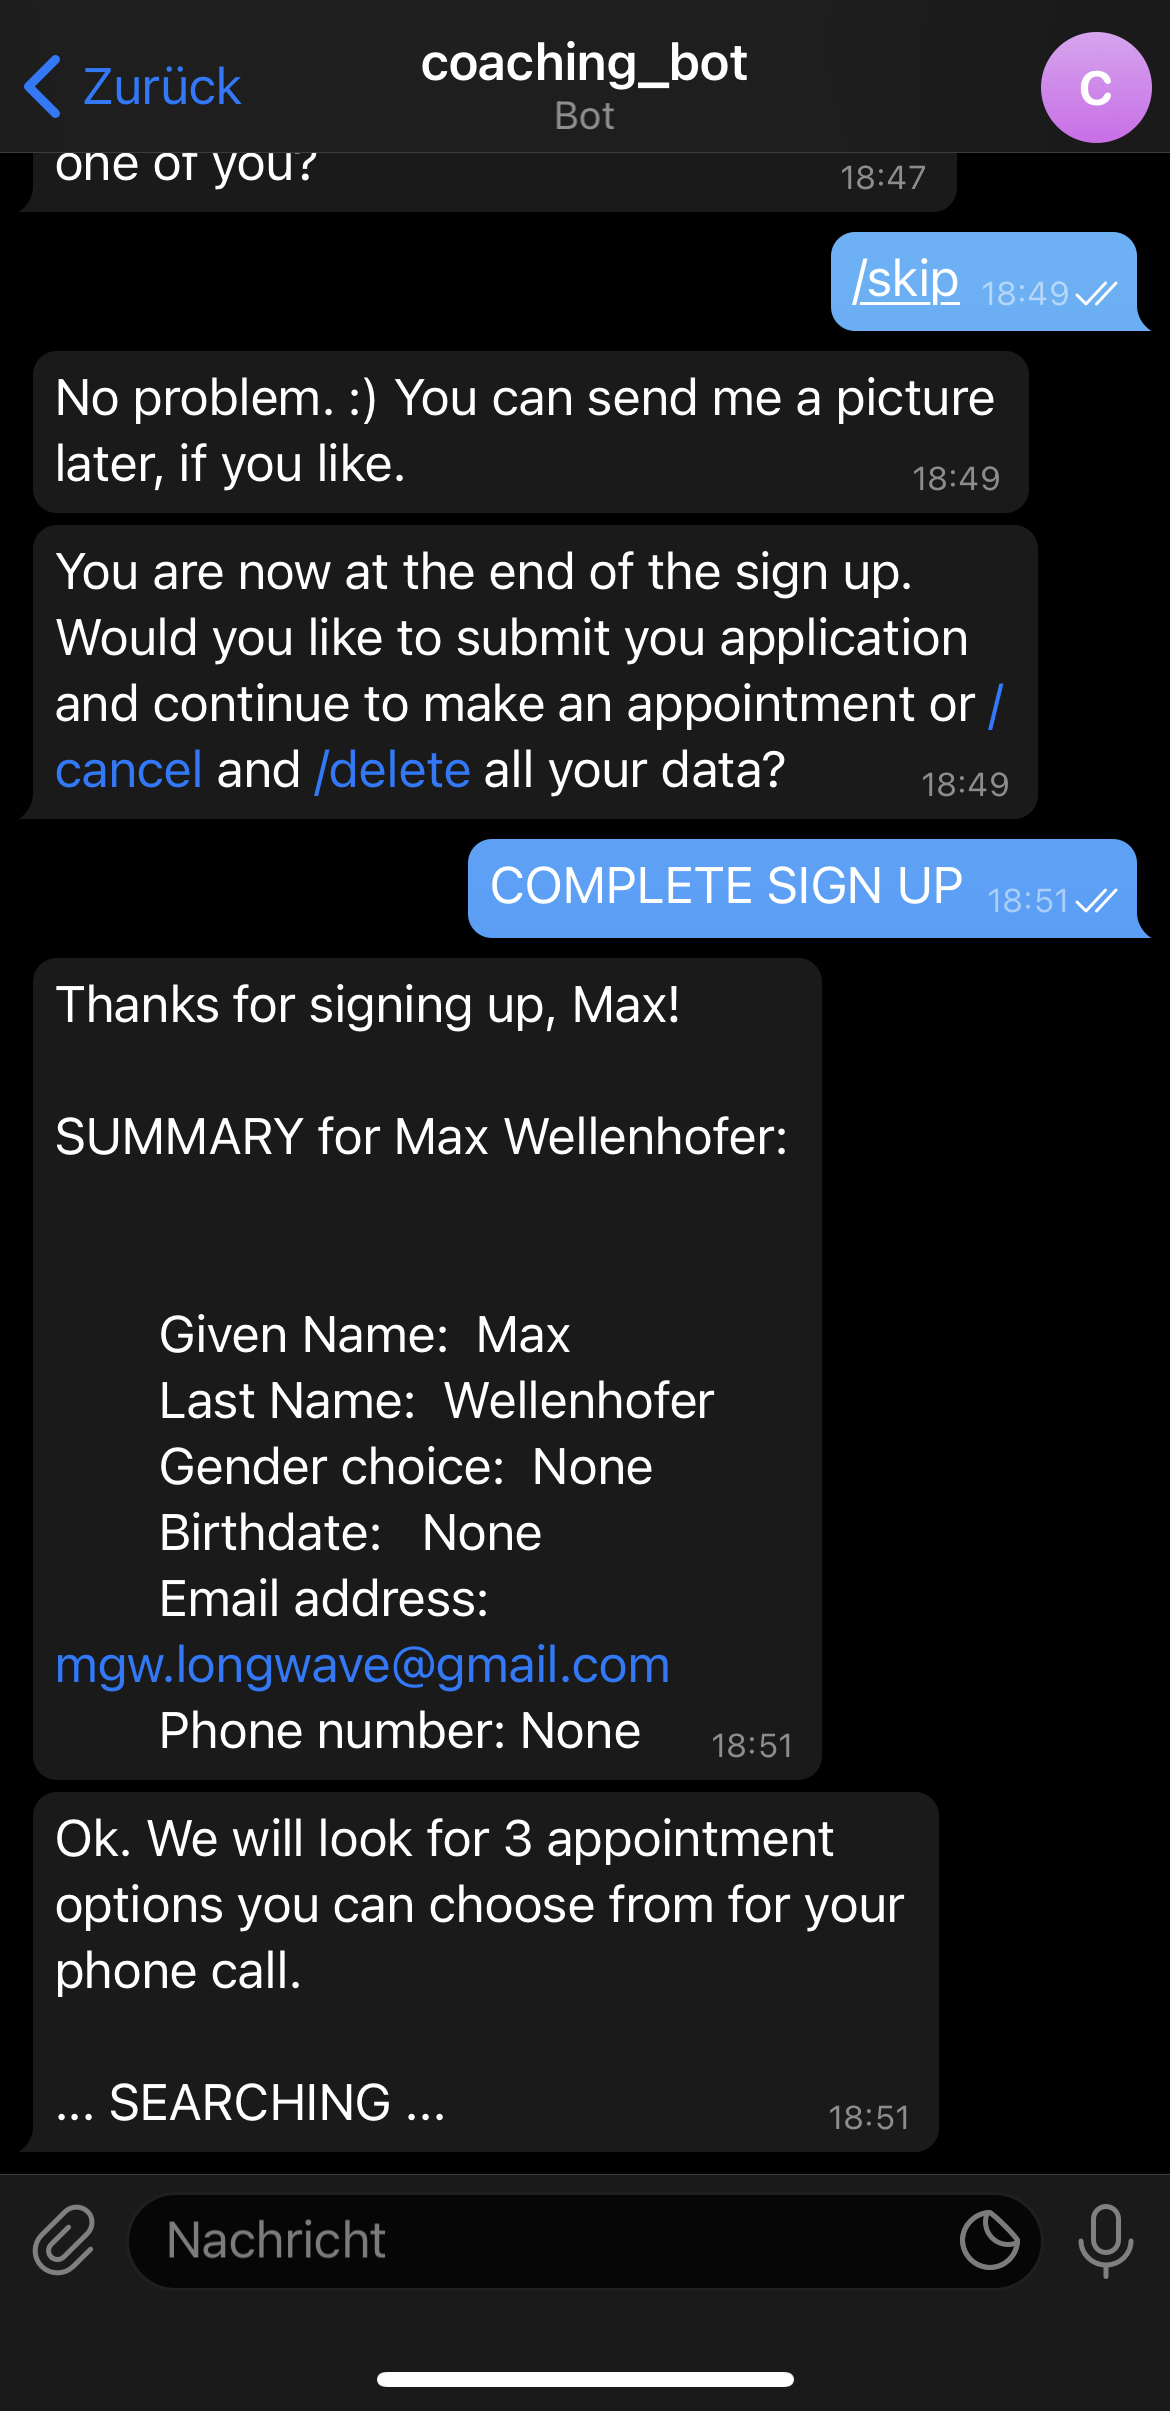
\includegraphics{images/coaching_bot_dummy_screenshot.jpeg}
	\caption{Bezeichnung der Abbildung}
	\label{a6}
\end{figure}


\subsection{Stage 06}
\begin{figure} %[hbtp]
	\centering
	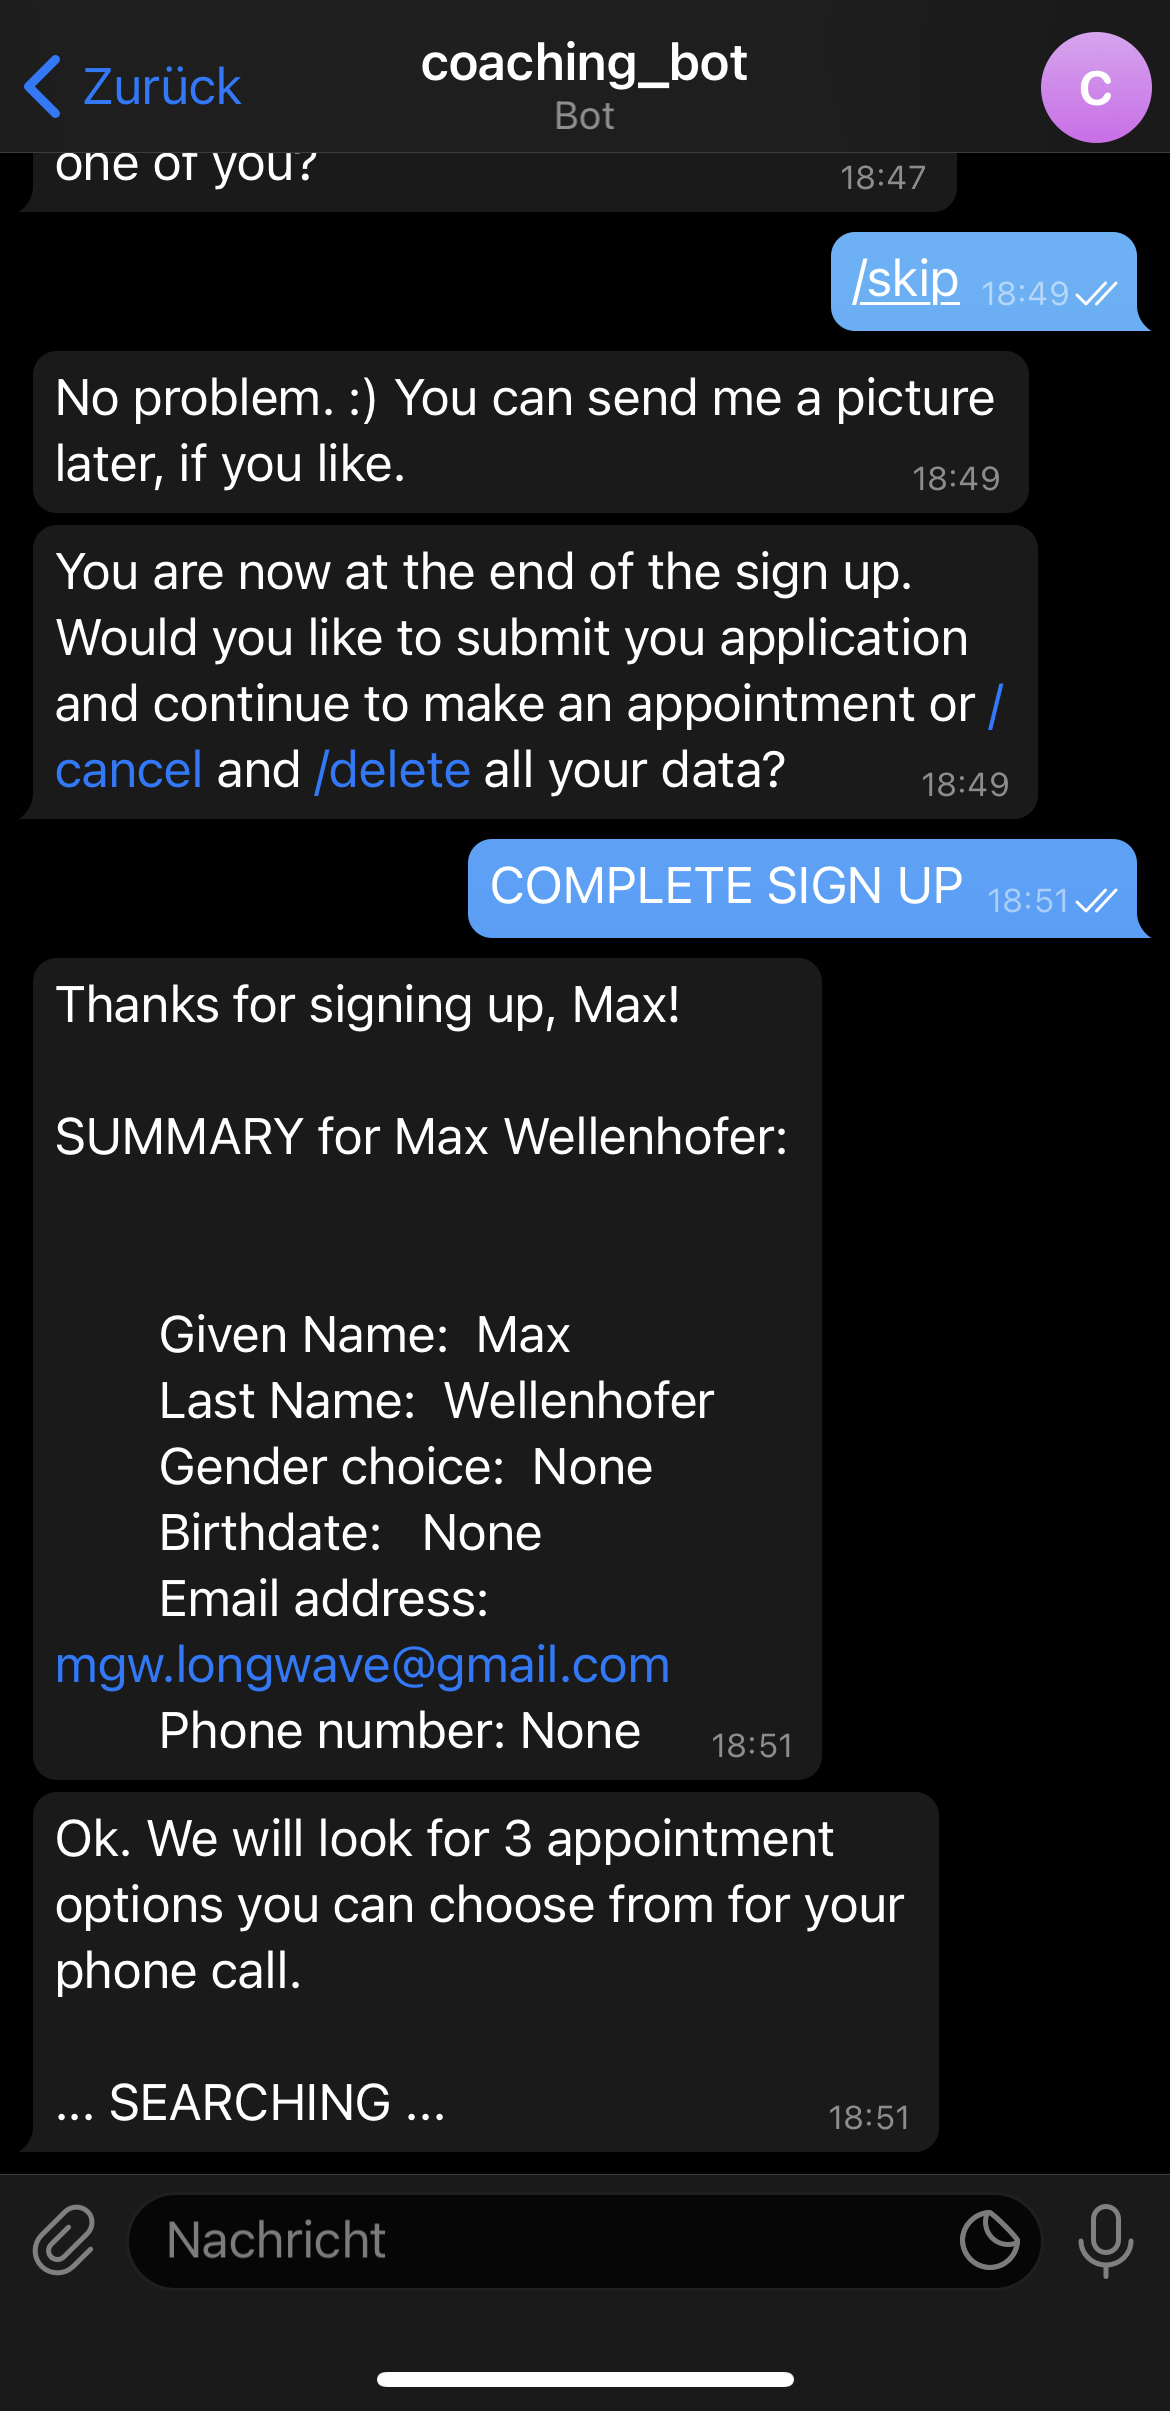
\includegraphics{images/coaching_bot_dummy_screenshot.jpeg}
	\caption{Bezeichnung der Abbildung}
	\label{a7}
\end{figure}


\subsection{Stage 07}
\begin{figure} %[hbtp]
	\centering
	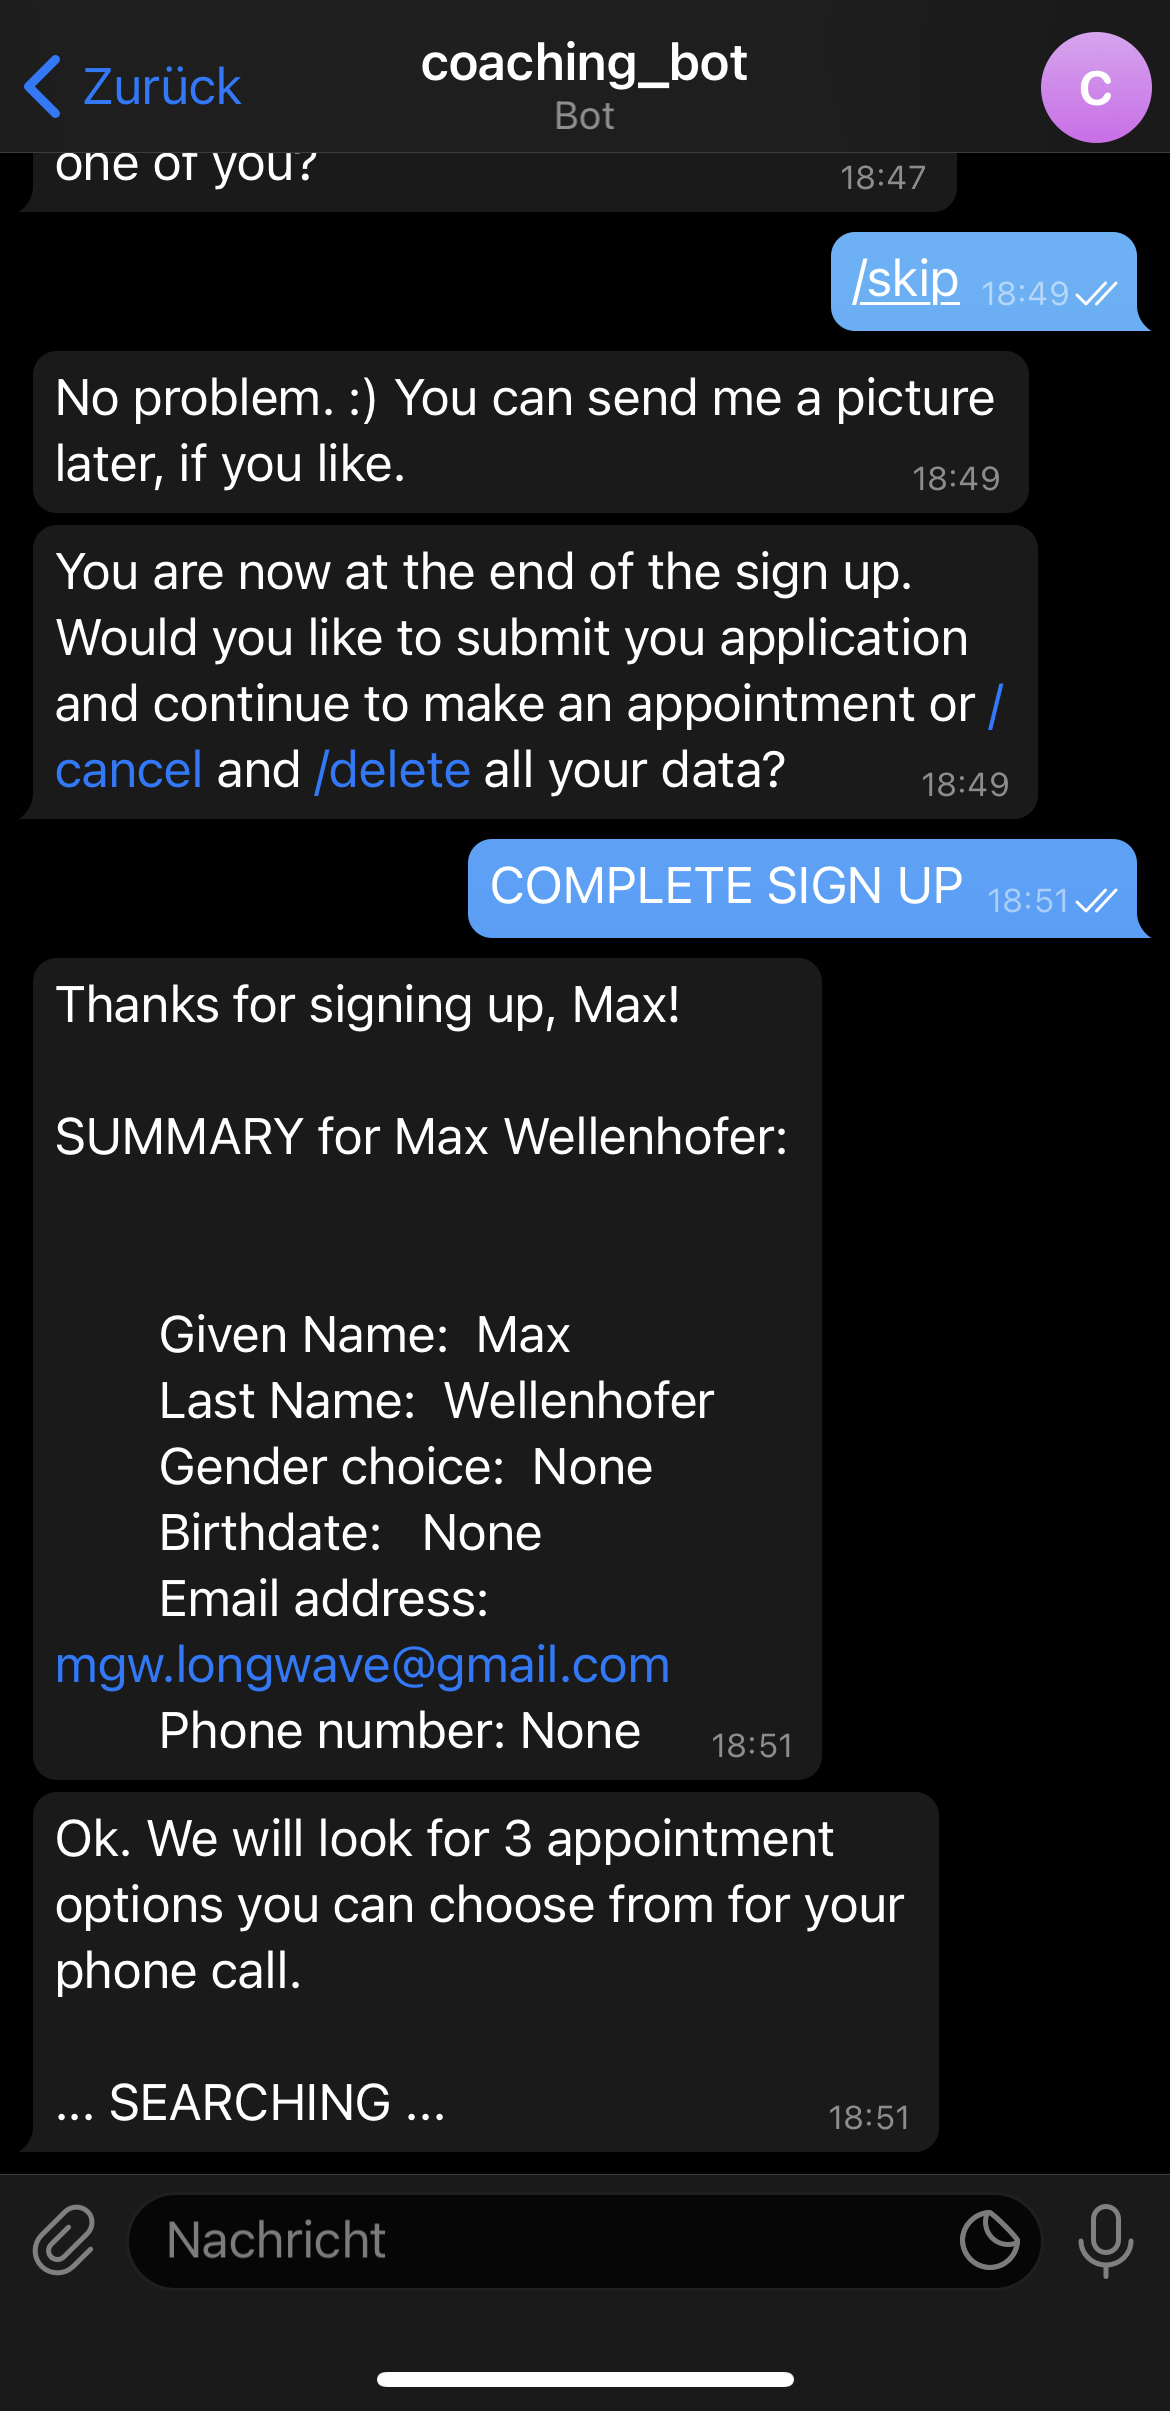
\includegraphics{images/coaching_bot_dummy_screenshot.jpeg}
	\caption{Bezeichnung der Abbildung}
	\label{a8}
\end{figure}


\subsection{Stage 08}
\begin{figure} %[hbtp]
	\centering
	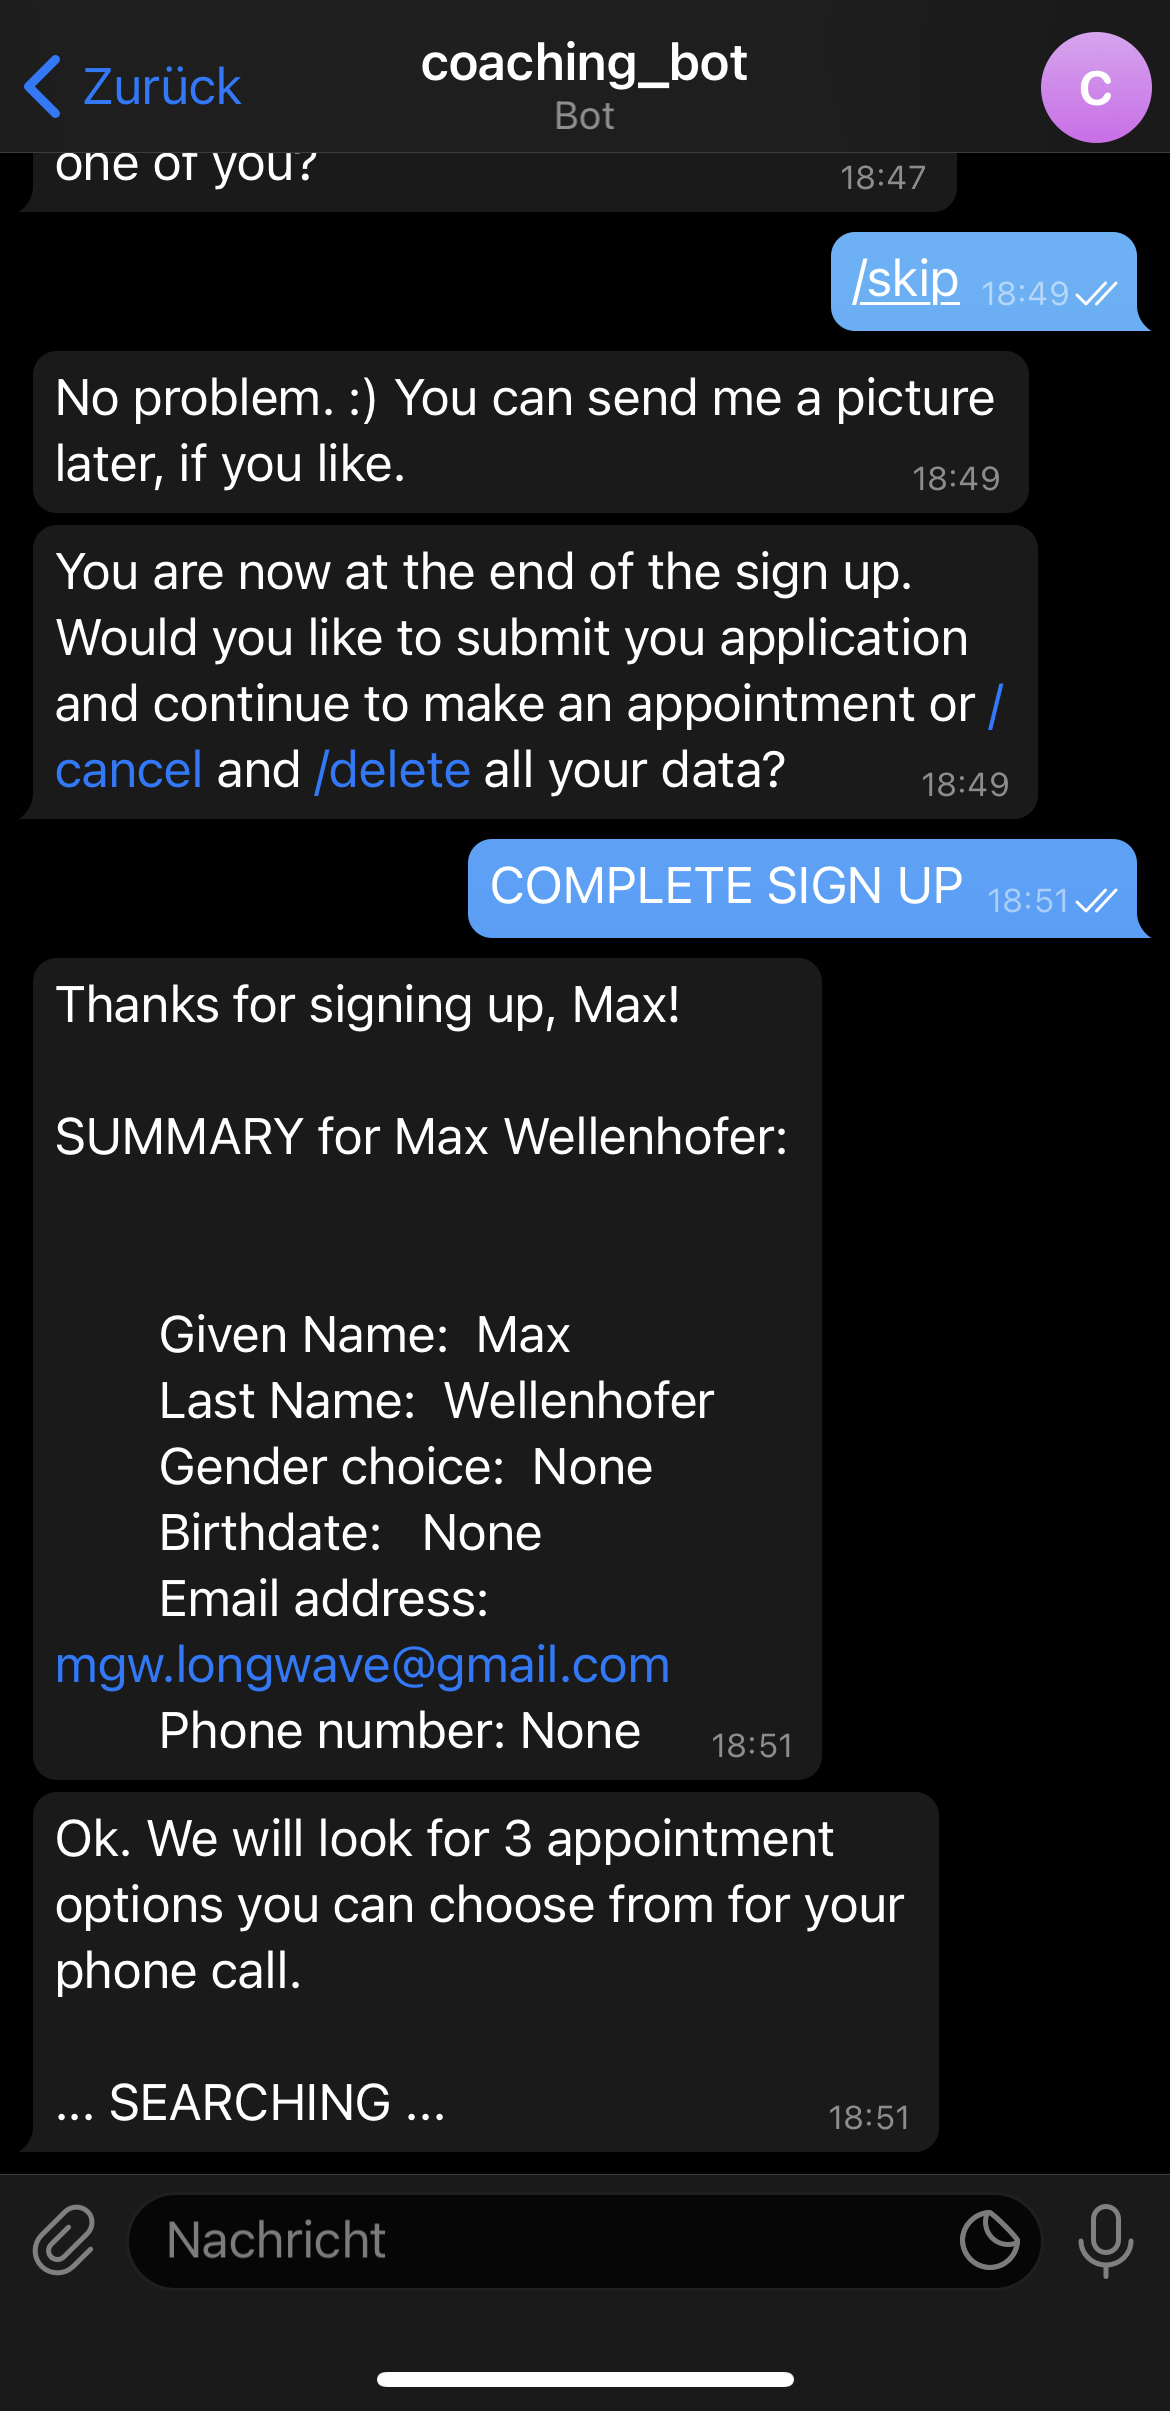
\includegraphics{images/coaching_bot_dummy_screenshot.jpeg}
	\caption{Bezeichnung der Abbildung}
	\label{a9}
\end{figure}


\subsection{Stage 09}
\begin{figure} %[hbtp]
	\centering
	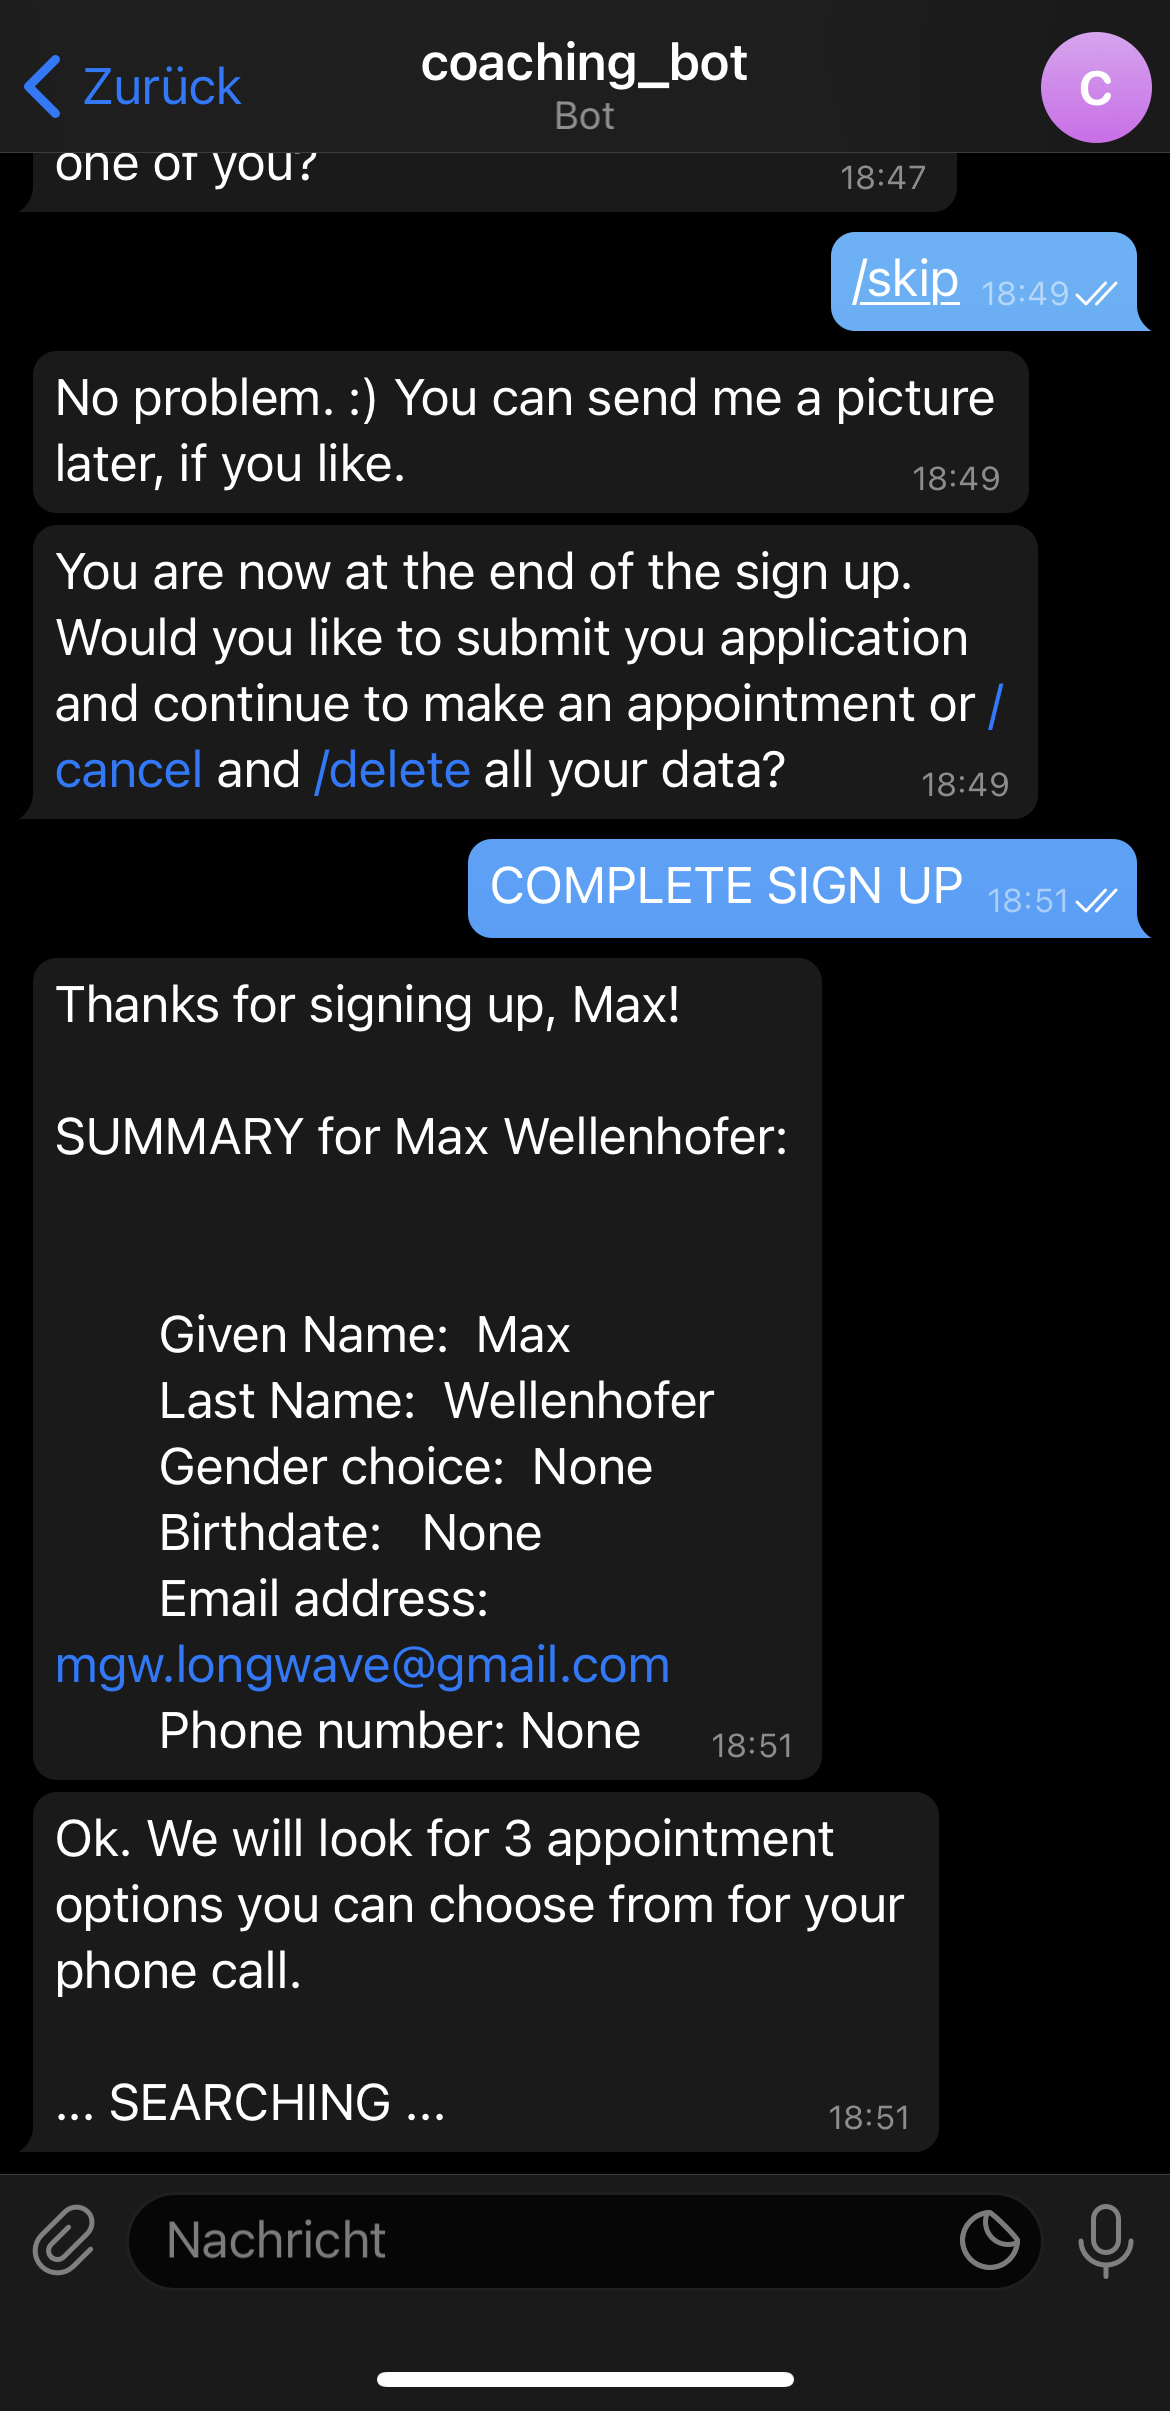
\includegraphics{images/coaching_bot_dummy_screenshot.jpeg}
	\caption{Bezeichnung der Abbildung}
	\label{a10}
\end{figure}

